\section{Moving Average Model}
\label{sec:MA}
Moving Average (MA) models are a type of model well-suited for univariate time series analysis. Unlike Autoregressive (AR) models, where the target variable depends directly on its past values, MA models rely on past random errors to predict future values.
Moreover, an important advantage of MA models compared to AR models is that MA models are guaranteed to be stationary. \\
The general formulation of a moving average model of order $q$ is given by:
\begin{equation}
    y_{t} = \mu_0 + \sum_{i=1}^{q} \theta_i \epsilon_{t-i} + \epsilon_{t}
\end{equation}
Here, $\mu_0$ represents the mean of the series, $\theta_1, ... , \theta_q$ are the model coefficients, and $\epsilon_t, \epsilon_{t-1}... , \epsilon_{t-q}$ are the error terms. \\
For our specific case, we implemented the model of order 1 ($q=1$) and order 2 ($q=2$). When $q=1$, the model is:
\begin{equation}
    \label{MA_q1}
    y_{t}=\mu_{0}+\theta \epsilon_{t-1} +\epsilon_t \qquad 
    \epsilon_t \stackrel{iid}{\sim} \mathcal{N}(0,\sigma^2)
\end{equation}
For $q=2$, the model becomes:
\begin{equation}
    \label{MA_q2}
    y_{t}=\mu_{0}+\theta_1 \epsilon_{t-1}+\theta_2 \epsilon_{t-2}+\epsilon_t   \qquad 
    \epsilon_t \stackrel{iid}{\sim} \mathcal{N}(0,\sigma^2)
\end{equation}
In both scenarios, the error terms are assumed to be independently and identically distributed (iid) following a normal distribution with mean 0 and variance $\sigma^2$.

\section*{MA(1)}
\label{MA(1)}
Referring to the formulation in \ref{MA_q1}, the likelihood is expressed as follows:
$$
y_t | \mu_0, \theta, \sigma^2, \epsilon_{t-1} \sim \mathcal{N}(\mu_0 + \theta \epsilon_{t-1},\sigma^2)
$$
And, the priors are:
\begin{equation}
    \begin{split}
        \mu_0 \sim \mathcal{N}(0.0, 10000) \\
        \tau = 1 / \sigma^2 \sim \mathcal{G}(2, 0.1) \\
        \theta \sim \mathcal{U}(-1.0, 1.0)
    \end{split}
\end{equation}
As we can notice, these priors have been chosen because they are uninformative. \\
Now, by running the JAGS code that implements the MA model of order 1 for the GDP and for the inflation, we obtain the following posteriors:
\begin{figure}[h]
    \centering
    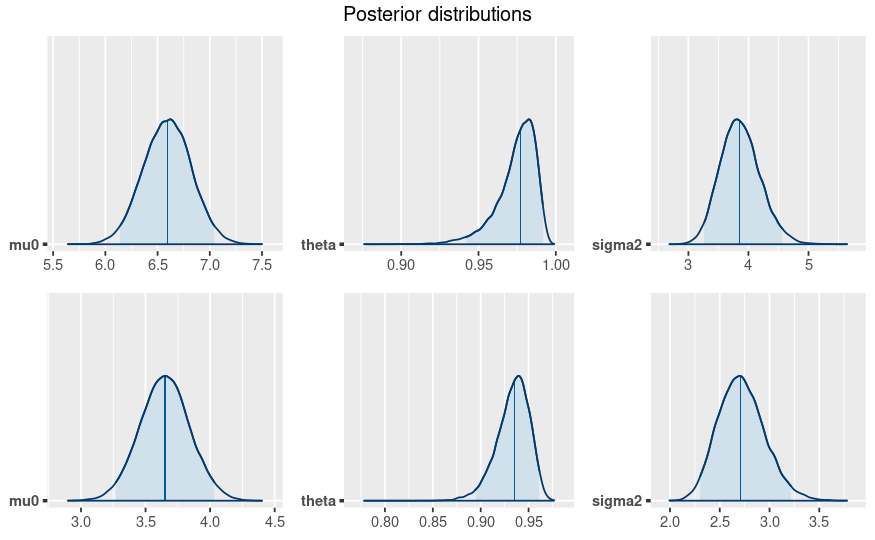
\includegraphics[width=\textwidth]{images/3-MA/posteriors.png}
    \caption{The image displays the posterior distributions of the parameters for the MA(1) model. The top line corresponds to the model used for GDP, while the bottom line corresponds to the model used for inflation.}
    \label{fig:MA_posteriors}
\end{figure}

\begin{figure}[h]
    \centering
    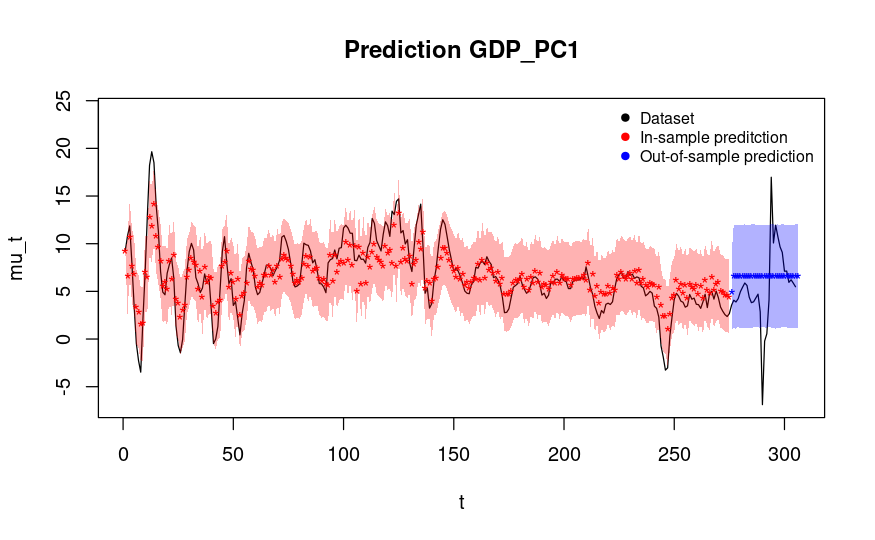
\includegraphics[width=\textwidth]{images/3-MA/gdp_prediction.png}
    \label{fig:MA_first}
\end{figure}
\begin{figure}[h]
    \centering
    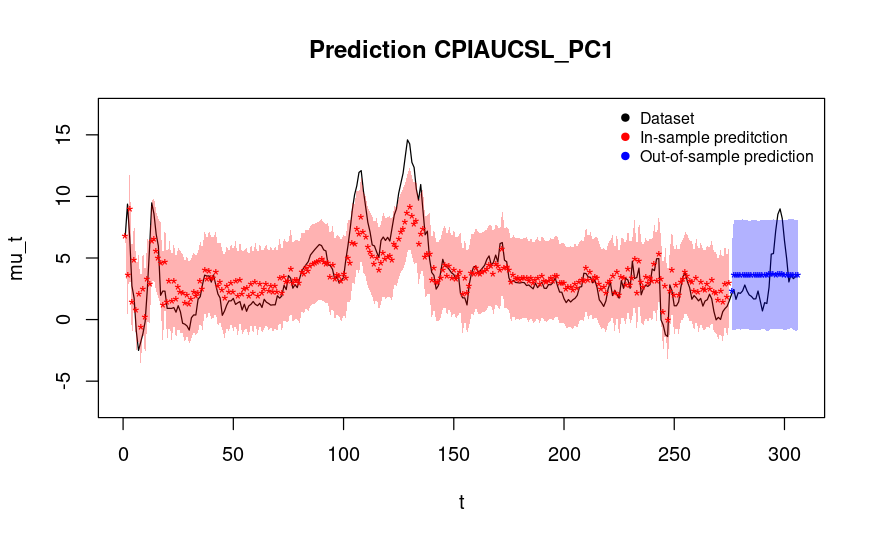
\includegraphics[width=\textwidth]{images/3-MA/infl_prediction.png}
    \label{fig:MA_second}
\end{figure}

\subsection*{MA(2)}
\label{MA(2)}
Referring to the formulation in \ref{MA_q2}, the likelihood is expressed as follows:
$$
y_t | \mu_0, \theta_1, \theta_2, \sigma^2, \epsilon_{t-1} \sim \mathcal{N}(\mu_0 + \theta_1 \epsilon_{t-1} + \theta_2 \epsilon_{t-2},\sigma^2)
$$
And, the priors are:
\begin{equation}
    \begin{split}
        \mu_0 \sim \mathcal{N}(0.0, 10000) \\
        \tau = 1 / \sigma^2 \sim \mathcal{G}(2, 0.1) \\
        \theta_1 \sim \mathcal{U}(-1.5, 1.5) \\
        \theta_2 \sim \mathcal{U}(-1.0, 1.0)
    \end{split}
\end{equation}

\begin{figure}[h]
    \centering
    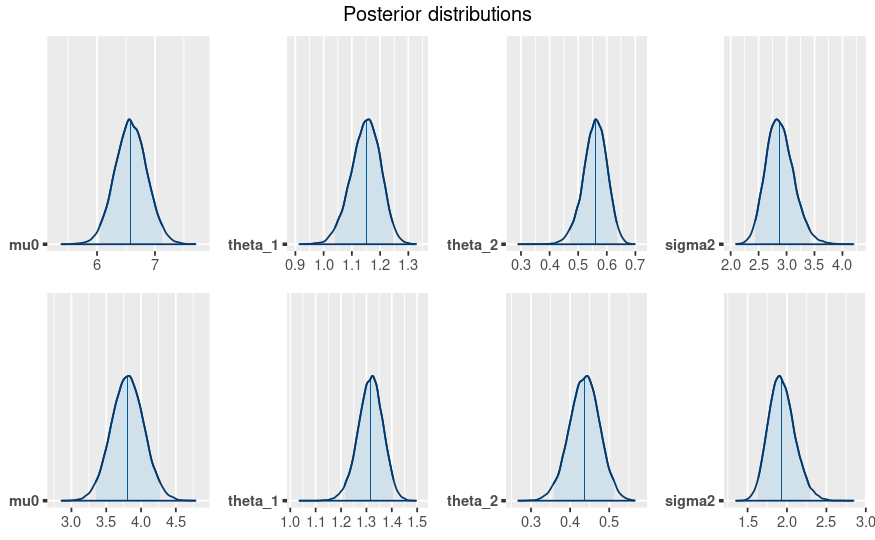
\includegraphics[width=\textwidth]{images/3-MA/posteriors2.png}
    \caption{The image displays the posterior distributions of the parameters for the MA(2) model. The top line corresponds to the model used for GDP, while the bottom line corresponds to the model used for inflation.}
    \label{fig:MA2_posteriors}
\end{figure}

\begin{figure}[h]
    \centering
    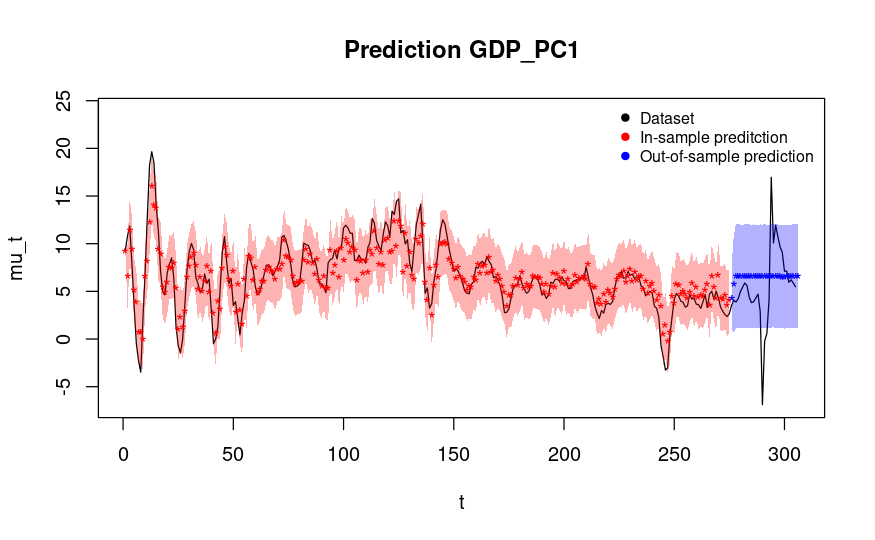
\includegraphics[width=\textwidth]{images/3-MA/gdp_prediction2.png}
    \label{fig:MA2_first}
\end{figure}
\begin{figure}[h]
    \centering
    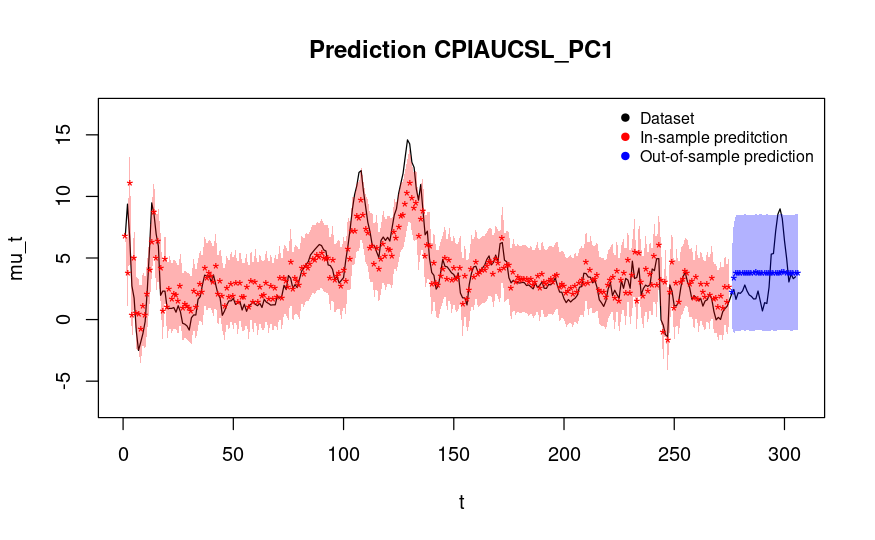
\includegraphics[width=\textwidth]{images/3-MA/infl_prediction2.png}
    \label{fig:MA2_second}
\end{figure}